\chapter{Grundlagen}
In diesem Kapitel werden das Vorgehensmodell und alle Tools, die für die erfolgreiche
Abwicklung des Projekts nötig sind, erläutert.

\section{Vorgehensmodelle}
Im Vorfeld der Durchführung des Projekts wurden Informationen über diverse Vorgehensmodelle
gesammelt. Für das Projektteam war schnell klar, dass ein agiles Modell gewählt werden sollte,
da somit das Projekt dynamischer geplant und durchgeführt werden kann. Die Auswahl für Scrum
stand direkt bei Projektbegin fest. In dem folgenden Abscnhitt wird dieses
Vorgehendsmodell genauer erklärt und unsere Entscheidung anschließend begründet.

\subsection{Scrum}
Scrum repräsentiert ein agiles Projektmanagement-Framework,
das auf die effiziente Entwicklung von Produkten und Software abzielt. Es legt besonderen Wert auf Zusammenarbeit,
Anpassungsfähigkeit und die kontinuierliche Bereitstellung funktionsfähiger Inkremente innerhalb kurzer Entwicklungszyklen,
den sogenannten Sprints.\footnote{Quelle: Scrum Alliance \cite{WHAT-IS-SCRUM}} \\

Die zuvor skizzierte Definition gewährt einen knappen Einblick in das agile Vorgehensmodell Scrum. Die herausragenden Merkmale dieses Modells sind:

\begin{itemize}
    \item Drei zentrale Rollen, die im Folgenden näher erläutert werden.
    \item Der Product Backlog, der sämtliche Anforderungen enthält.
    \item Eine iterative und zeitlich definierte Entwicklung von Produkten.
    \item Die autonome Arbeitsweise des Teams.
    \item Gleichberechtigung aller Teammitglieder.
\end{itemize}

\subsection{Die drei Rollen in Scrum}
\begin{itemize}
    \item \textbf{Product Owner}: Der Product Owner trägt die Verantwortung
    für die Pflege des Product Backlogs und vertritt dabei die fachliche Auftraggeberseite sowie sämtliche Stakeholder.
    Ein zentrales Anliegen ist die Priorisierung der Elemente im Product Backlog, um den geschäftlichen Wert des
    Produkts zu maximieren und die Möglichkeit für frühe Veröffentlichungen essenzieller Funktionalitäten zu schaffen.
    Der Product Owner nimmt nach Möglichkeit an den täglichen Scrum-Meetings teil, um auf passive Weise Einblicke zu
    gewinnen. Zudem steht er dem Team für Rückfragen zur Verfügung, um einen reibungslosen Informationsaustausch zu gewährleisten.\footnote{Scrum-Rolle \cite{Product-Owner}}
    \item \textbf{Scrum Master}: Der Scrum Master übernimmt eine zentrale
    Rolle im Scrum-Prozess und ist für die korrekte Umsetzung desselben verantwortlich. Als Vermittler und Unterstützer
    fungiert er als Facilitator, der darauf abzielt, einen maximalen Nutzen zu erzielen und kontinuierliche Optimierung
    sicherzustellen. Ein zentrales Anliegen ist die Beseitigung von Hindernissen, um ein reibungsloses Voranschreiten
    des Teams zu gewährleisten. Der Scrum Master sorgt für einen effizienten Informationsfluss zwischen dem Product Owner
    und dem Team, moderiert Scrum-Meetings und behält die Aktualität der Scrum-Artefakte wie Product Backlog,
    Sprint Backlog und Burndown Charts im Blick. Darüber hinaus liegt in seiner Verantwortung, das Team vor
    unberechtigten Eingriffen während des Sprints zu schützen.\footnote{Scrum-Rolle \cite{Scrum-Master}}
    \item \textbf{Team}: Das Team, bestehend aus vier bis zehn Mitgliedern,
    idealerweise sieben, zeichnet sich durch eine interdisziplinäre Zusammensetzung aus, die Entwickler, Architekten,
    Tester und technische Redakteure einschließt. Durch Selbstorganisation agiert das Team eigenständig und übernimmt
    die Verantwortung als sein eigener Manager. Es besitzt die Befugnis, autonom über die Aufteilung von Anforderungen
    in Aufgaben zu entscheiden und diese auf die einzelnen Mitglieder zu verteilen, wodurch der Sprint Backlog aus dem
    aktuellen Teil des Product Backlog entsteht.\footnote{Scrum-Rolle \cite{Team}}
\end{itemize}
\\
Alle Anforderungen an das Produkt werden in sogenannten User Stories, vorrangig erstellt durch den Product
Owner, im Product Backlog gesammelt. In einem Intervall, bezeichnet als Sprint, werden die User Stories abgearbeitet.
Die Projektentwicklung nach Scrum besteht aus fünf zentralen Elementen:
\begin{itemize}
    \item \textbf{Sprint: Planning Meeting}: Im Sprint Planning
    Meeting wird das Ziel des folgenden Sprints definiert. Hierbei werden die Anforderungen im Project Backlog, die in
    diesem Sprint umgesetzt werden sollen, in einzelne Aufgaben zerlegt und anschließend im Sprint Backlog gesammelt.\footnote{Scrum-Meetings \cite{Sprint-planing-meeting}}
    \item \textbf{Sprint}: Ein Sprint repräsentiert eine Entwicklungsphase,
    während der eine voll funktionsfähige und potenziell veröffentlichte Software entsteht. Die Dauer eines solchen
    Sprints beträgt typischerweise zwischen 1 und 4 Wochen.\footnote{Scrum-Meetings \cite{Sprint}}
    \item \textbf{Daily Scrum}: Der Daily Scrum ist ein kurzes Teammeeting,
    in dem Teammitglieder darüber informieren, welche Aufgaben seit dem letzten Meeting abgeschlossen wurden, woran bis
    zum nächsten Meeting gearbeitet werden muss und wo momentane Probleme existieren. Auf diese Weise sind alle Teammitglieder
    stets auf dem aktuellen Stand, was die Lösung aufkommender Probleme erleichtert. \footnote{Scrum-Meetings \cite{Daily-Scrum}}
    \item \textbf{Sprint Review}: In diesem Meeting präsentiert das
    Entwicklungsteam die im Sprint abgeschlossenen Arbeitsergebnisse, beispielsweise fertige Produktinkremente, den
    Stakeholdern, zu denen Produktbesitzer, Kunden, Führungskräfte und andere Interessengruppen gehören.\footnote{Scrum-Meetings \cite{Sprint-Review}}
    \item \textbf{Sprint Retrospective}: Die Sprint Retrospective
    dient primär dazu, dass das Scrum-Team (bestehend aus dem Entwicklungsteam, dem Scrum Master und dem Product Owner)
    gemeinsam den abgeschlossenen Sprint reflektiert und Möglichkeiten zur kontinuierlichen Verbesserung identifiziert.\footnote{Scrum-Meetings \cite{Sprint-Retroperspektiv}}
\end{itemize}

Durch diese Elemente kann ein optimaler Projektablauf gewährleistet werden. Das Projekt bleibt jederzeit
offen für Änderungen, und durch eine enge Zusammenarbeit mit dem Kunden können Missverständnisse und Probleme
frühzeitig behandelt und kommuniziert werden.

\subsection{Begründung der Auswahl}
Die Applied Augmented Reality in Education Applikation besteht aus 3 verschiedenen Level.
Im Team welches aus vier Schülern bestand übernahm jede Person einen Teilbereich oder arbeiteten
gemeinsam an einem dieser Level mit Unteraufgaben in diesem Level. Unterstützt wurde man von einem
Lehrer, der stetz für Fragen bereitstand und oftmals in beratender Form vorhanden war. Als
Vorgehensmodell wählte das Team das agile Modell Scrum. Die von Scrum gegebenen Richtlinien
konnten leicht eingehalten werden, da das Team täglich in der Schule aufeinander
traf als auch privat Kontakt hatten. Jederart Änderung, Problem oder Änderungen und anderartige
Dinge konnten daher leicht kommuniziert und besprochen werden. Am Ende jedes Sprints wurden
die erreichten Ergebnisse mit dem Betreuer besprochen, sowie die Neuerungen vorgestellt.
In den Sprintreviews konnte somit Feedback zu den Ergebnissen gesammelt werden und von dem
Betreuer konnten neue Ansichten und Denkweisen angebracht und integriert werden.
Durch die Sprint Retroperspektive konnten die Schüler einen größeren Mehrwert aus der
Projektentwicklung schöpfen, da sie neben der Verwendung des Scrum-Prozesses auch ihre Fähigkeiten
in den einzelnen Bereichen, durch das Besprechen der positiven und negativen Aspekte verbessern.

\section{Projektmanagement-Tools}
Um einen positiven Verlauf des Projekts zu ermöglichen, benötigt man die unterstützenden
Tools beim Projektmanagement sowie die Verwaltung von Dateien.

\subsection{GitHub}
Als sogenanntes Repository für die Source Code Dateien wurde GitHub mit der dazugehörigen
Webanwendung verwendet. Zu Beginn des Projekts stand die Entscheidung an, welche Technologie
und welcher Anbieter für das Versionskontrollsystem gewählt werden sollten. Neben GitHub gibt es
andere namhafte Anbieter solcher Verwaltungssysteme, darunter GitLab und SourceForge.

Ausschlaggebend für die Wahl von GitHub waren mehrere Punkte. Zum einen ist GitHub eine
kostenlose Lösung, die es ermöglicht, ein privates Projekt mit mehreren Mitgliedern
ohne Kosten anzulegen. Im Gegensatz dazu bieten manche Plattformen nur eine begrenzte Anzahl
von Mitgliedschaften in kostenfreien Projekten an. Die Registrierung erforderte lediglich
einen Account.

Darüber hinaus bietet GitHub eine benutzerfreundliche Oberfläche, eine breite Unterstützung
für verschiedene Programmiersprachen und eine aktive Entwicklergemeinschaft. Dies erleichtert
die Zusammenarbeit und den Informationsaustausch im Projektteam.

\subsection{Jira}
Als sogenanntes Verwaltungstool für die Vorgänge im Projekt wurde Jira mit der dazugehörigen
Webanwendung verwendet. Auch hier stand zu Projektbeginn die Frage im Raum, welche Technologie
und welcher Anbieter für das Aufgabenmanagement gewählt werden sollten. Neben Jira gibt es
weitere namhafte Anbieter solcher Tools, darunter VivifyScrum und KanBan.

Die Wahl von Jira basierte auf mehreren Überlegungen. Zum einen ist Jira eine kostenlose
Lösung, die es ermöglicht, ein SCRUM Board mit mehreren Mitgliedern kostenfrei anzulegen.
Ein weiterer entscheidender Faktor war die direkte Verbindung zu dem GitHub-Repository und die Möglichkeit,
neue Branches und Commits direkt in Jira zu erstellen.

Darüber hinaus bietet Jira eine umfassende Funktionalität für das Projektmanagement, einschließlich
der Verfolgung von Aufgaben, der Planung von Sprints und der Erstellung von Berichten. Diese Features
ermöglichen es dem Projektteam, den Fortschritt genau zu überwachen und eventuelle Herausforderungen
frühzeitig zu identifizieren und anzugehen.

\section{Konzeption von Fragebögen}
Bei jeder Umfrage werden Informationen von Personen oder Personengruppen zu der allgemeinen
Umsetzung und dem Verständis der Applikation gesammelt. Diese werden im Anschluss ausgewertet und
interpretiert. Wichtig ist hier den Zweck jeder Umfrage genau zu definieren. Durch präzise und
detailierte Zielsetzungen ist es später dann möglich, den Erfolg der Umfrage zu garantieren.

\subsection{Planung der Fragebogenkonstruktion}

Die sorgfältige Konzeption und Gestaltung eines Fragebogens sind grundlegende Schritte, die bei der Planung einer Erhebung unternommen werden.
Durch eine sorgfältige Planung wird sichergestellt, dass relevante Daten erhoben werden und die spätere Auswertung erleichtert wird.
Aus diesem Grund müssen bereits im Vorfeld verschiedene Entscheidungen getroffen und Definitionen festgelegt werden:

\begin{enumerate}

    \item \textbf{Inhalt}\\
    Die Auswahl der Inhalte ist für die Qualität der erhobenen Daten entscheidend. Es sollte erwogen werden, bestehende
    Fragebögen zu verwenden und gegebenenfalls an die spezifischen Anforderungen der Erhebung anzupassen. Um Missverständnisse
    zu vermeiden, sollten die Fragen klar und prägnant formuliert sein. Die Verwendung validierter Fragebögen kann bei der
    Gewährleistung der Vergleichbarkeit mit anderen Studien hilfreich sein.

    \item \textbf{Umfang}\\
    Ein wichtiger Faktor, der je nach Forschungsziel abgewogen werden muss, ist die Länge des Fragebogens. Das Ziel sollte
    ein ausgewogenes Verhältnis zwischen der Tiefe der Informationen und der Aufrechterhaltung der Teilnahme der Teilnehmer
    sein. Ein zu umfangreicher Fragebogen kann dazu führen, dass die Befragten ermüden und die Qualität der Antworten
    beeinträchtigt wird.

    \item \textbf{Ablauf und zeitlicher Rahmen}\\
    Die Entscheidung bezüglich des Ablaufs und des Zeitrahmens der Befragung beeinflusst die Art der Datensammlung. Die
    Wahl zwischen einer postalischen und einer elektronischen Befragung wirkt sich auf die Antwortzeit und die Effizienz
    der Datenerhebung aus. Bei elektronischen Erhebungen liegen die Ergebnisse oft schneller vor, während bei postalischen
    Erhebungen längere Antwortzeiten möglich sind.

    \item \textbf{Zielgruppe}\\
    Die Definition der Zielgruppe spielt eine wichtige Rolle für die Repräsentativität der Ergebnisse. Die Entscheidung
    für eine Vollerhebung oder eine Stichprobe ist eine Frage der zur Verfügung stehenden Ressourcen und der spezifischen
    Forschungsziele. Eine Vollerhebung kann eine umfangreiche Datenbasis liefern, während eine Stichprobenerhebung
    insbesondere bei großen Zielgruppen effizienter sein kann.

    \item \textbf{Fragetypen und Antwortskalen}\\
    Die Qualität der erhobenen Daten wird durch die Wahl der Art der Fragen und die Wahl der Antwortskalen beeinflusst.
    Geschlossene Fragen mit vorgegebenen Antwortmöglichkeiten erleichtern die quantitative Analyse, während offene Fragen
    die Möglichkeit bieten, qualitative Einsichten zu gewinnen. Die Wahl der Antwortskalen, unabhängig davon, ob es sich
    um Likert-Skalen oder numerische Bewertungen handelt, sollte auf die spezifischen Forschungsziele abgestimmt sein.

    \item \textbf{Ethik und Datenschutz}\\
    Es ist von entscheidender Bedeutung, ethische Aspekte zu berücksichtigen, wie die Anonymität der Teilnehmer zu wahren
    und sensible Informationen zu schützen. Der Fragebogen sollte so konzipiert sein, dass die Integrität der Teilnehmer
    geschützt wird und keine unangebrachten persönlichen Informationen gesammelt werden.

    \item \textbf{Pilotstudie}\\
    Es empfiehlt sich, vor der endgültigen Implementierung des Erhebungsbogens eine Pilotstudie durchzuführen. Im Rahmen
    dieser Testphase können mögliche Probleme, Unklarheiten oder Missverständnisse bei der Formulierung der Fragen erkannt
    und behoben werden. Das Feedback der Testteilnehmer trägt dazu bei, den Fragebogen noch weiter zu optimieren.
\end{enumerate}
\\

Um das Verständnis für die Gestaltung der Fragebögen und für die Formulierung der Fragen zu erleichtern, wird in diesem
Abschnitt ein \textit{Fallbeispiel} vorgestellt, auf das bei der weiteren Erläuterung zurückgegriffen wird.
\begin{quote}
    Während des Tages der offenen Tür im Schuljahr 2023/2024 (25 Personen) und in einer Abschlussklasse (14 Personen)
    einer Schule mit Matura wurde eine Umfrage durchgeführt, um die Nutzermeinungen zur aktuellen Anwendung zu erfassen.
    Das Ziel dieser Umfrage bestand darin zu ermitteln, ob die zugrunde liegenden Konzepte verstanden wurden und ob
    potenzielle Verbesserungsmöglichkeiten vorliegen. Eine quantitative Analyse hat ergeben, dass etwa ein Drittel der
    Teilnehmer des Tages der offenen Tür die Konzeptionen verstanden hat und keine spezifischen Verbesserungsvorschläge
    geäußert hat.

    Anschließend wurden vier Personen (Stichprobe) der Abschlussklasse befragt, um potenzielle Verbesserungsvorschläge
    zu ermitteln. Das Ziel dieser Umfragen bestand darin, Personen zu befragen, die bereits über grundlegendes IT-Wissen
    verfügen und dadurch besser beurteilen können, welche Aspekte verbessert werden können. Die Ergebnisse zeigen, dass
    die vermittelten Konzepte verstanden wurden. Allerdings wurden am Tag der offenen Tür im Vergleich zu den befragten
    Personen viele Verbesserungsvorschläge geäußert. Die Befragten gaben an, dass diese Vorschläge aufgrund des frühen
    Entwicklungsstadiums der Anwendung entstanden sind und einige essenzielle Aspekte noch nicht oder nur teilweise
    implementiert waren, wodurch sie unklar blieben.
\end{quote}
\\

Grundsätzlich werden die \textit{quantitative} und die \textit{qualitative Forschung} unterschieden, wobei Fragebögen zur
\textit{quantitativen Forschung} aufgrund der besseren Vergleichbarkeit leichter zu interpretieren sind.

Bei der Quantifizierung schließt man von der Stichprobe auf die Grundgesamtheit N, wie in Abbildung \ref{fig:GrundgesamtheitStichprobe}
gezeigt. Es ist wichtig, dass die ausgewählte Stichprobe repräsentativ ist. Das bedeutet, dass die Personen, die an der
Stichprobe teilnehmen, die gleichen Voraussetzungen haben wie die Personen, die tatsächlich in der Grundgesamtheit vorkommen.
Es handelt sich hierbei um numerische Daten, die erhoben werden und für die eine Auswertung vorgenommen wird. Von Bedeutung
ist in diesem Zusammenhang das Verhältnis zwischen der untersuchten Stichprobe und der Grundgesamtheit (Population). In
diesem Zusammenhang ist das Verhältnis zwischen der untersuchten Auswahl und der Population von Bedeutung. Alle Merkmale
der Personen in der Auswahl müssen mit den Merkmalen der Personen in der Population übereinstimmen, zum Beispiel Alter
und Geschlecht.\footnote{Vgl. Mayer, \cite{Interview und schriftliche Befragung}, S. 57 ff.}

%Hier Bild für den Zusammenhand
\begin{figure}[h]
    \centering
    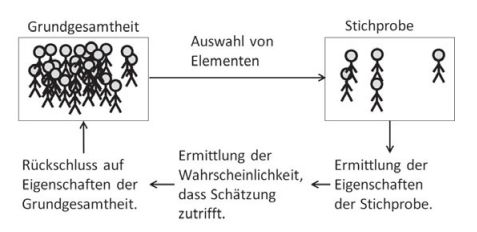
\includegraphics[width=1\textwidth]{images/zsmhGrundStich}
    \caption{Zusammenhang zwischen der \textit{Grundgesameheit} und \textit{Stichprobe}}
    \label{fig:GrundgesamtheitStichprobe}
\end{figure}

Anhand des Fallbeispiels wird verdeutlicht, dass es keinen Sinn macht, die Umfrage an sehr jungen Leuten durchzuführen,
da diese Personen zum größten Teil noch nicht wirklich tiefer in die Informatik geblickt haben und dadurch keinerlei
Verbesserungsvorschläge geben können.

Die qualitative Forschung ist eine Methode zur Auswertung von Daten, die ausschließlich über Sprache (verbal) übermittelt
werden. Diese Methode eignet sich vor allem zur näheren Beschreibung und Analyse von subjektiven Wahrnehmungen, persönlichen
Einstellungen, Motiven und Meinungen der Befragten.\footnote{Vgl. Mayer, \cite{Interview und schriftliche Befragung}, S. 36}

Am sinnvollsten ist eine Kombination von \textit{qualitativen und quantitativen Ergebnissen}. Nach einer quantitativen
Befragung sollte eine stichprobenartige qualitative Befragung durchgeführt werden, um die Ergebnisse besser interpretieren
zu können. Dies wird anhand eines Fallbeispiels veranschaulicht.

Unabhängig davon, ob es sich um qualitative oder quantitative Forschung handelt, sind die drei \textit{Gütekriterien
Objektivität, Zuverlässigkeit und Validität} zu erfüllen.

Sie dienen, den Forschungsprozess zu steuern und zu kontrollieren. Die Validität ist ein Maß für die Brauchbarkeit der
Methode und bezieht sich auf die tatsächliche Fähigkeit zur Messung des gewünschten Wertes. Das Ergebnis ist umso zuverlässiger,
je klarer die Fragen formuliert sind. Entscheidend für die Validität der Analyse ist die Objektivität der Messung. Dabei
ist sowohl die Durchführungsobjektivität des Befragers als auch die Auswertungs- und Interpretationsobjektivität des
Analytikers zu beachten.\footnote{Vgl. Mayer, \cite{Interview und schriftliche Befragung}, S. 54 ff., S. 88.}

Die drei Gütekriterien stehen in einem wechselseitigen Zusammenhang. Nur, wenn die Objektivität gegeben ist, kann die
Reliabilität gewährleistet werden. Ist die Reliabilität gering, kann die Validität nur mit einer gewissen Unsicherheit
vorhergesagt werden.\footnote{Vgl. Bühner, \cite{Einfuehrung in die Test- und Fragebogenkonstruktion}, S. 33 f.}

\subsection{Formulierung der Fragen}
Um eine erfolgreiche Umfrage effizient durchführen zu können, ist eine sorgfältige Vorbereitung erforderlich. Die
Erkenntnis, dass Umfragen nur bestimmte Aspekte eines Themenbereichs abdecken können, ist von entscheidender Bedeutung.
Aus diesem Grund ist eine sorgfältige und präzise Definition dieser Aspekte erforderlich. Besonderes Augenmerk ist darauf
zu richten, dass die Fragen klar formuliert sind.

Die zentrale Priorität bei der Formulierung der Fragen ist die Verständlichkeit und Eindeutigkeit. Die folgenden
Formulierungsrichtlinien sollten unbedingt beachtet werden:
\begin{itemize}
    \item Verwendung von einfachem Vokabular ohne Verwendung von Fachausdrücken, Fremdwörtern oder Ausdrücken aus anderen Sprachen.
    \item Die Fragen prägnant formulieren.
    \item Belastende Begriffe wie \textit{Ehrlichkeit} werden vermieden.
    \item Hypothetische Formulierungen sollten ausgeschlossen werden.
    \item Fokussierung auf ein bestimmtes Thema für jede einzelne Frage.
    \item Vermeidung von Überforderung durch die Bereitstellung einer angemessenen Menge an Informationen pro Frage.
    \item Doppelte Verneinungen sind zu vermeiden.\footnote{Vgl. Mayer, \cite{Interview und schriftliche Befragung}, S. 89.}\\
\end{itemize}

Die genannten Kriterien sind besonders wichtig bei schriftlichen Befragungen. Um sicherzustellen, dass die Ergebnisse nicht
verfälscht werden, darf der Interviewer keine zusätzlichen Fragen stellen oder die bereits gestellten Fragen ändern.

Direkte Fragen sind geeignet, um Fakten und Wünsche zu ermitteln, während formulierte Aussagen oder Feststellungen eher
dazu dienen, die Bewertung durch die Befragten in Erfahrung zu bringen. Diese Techniken werden hauptsächlich zur Erfassung
von Einstellungen, Wahrnehmungen und Meinungen eingesetzt.

\subsection{Arten von Fragen}
In Abhängigkeit von den Anforderungen der jeweiligen Evaluation können sowohl offene als auch geschlossene Fragen gestellt werden.

Bei offenen Fragen handelt es sich um Fragen, bei denen keine Antwortmöglichkeiten vorgegeben werden. Im Anschluss an die
Frage sollte ausreichend Platz für die Beantwortung der Frage gelassen werden. Dieser Fragetyp sollte in den folgenden
Fällen verwendet werden:
\begin{itemize}
    \item Wenn die Anzahl der Antwortmöglichkeiten unbekannt ist.
    \item Wenn die Formulierung der Antwort des Auskunftspflichtigen für die Auswertung von Bedeutung ist.
    \item Wenn das Ziel der Erhebung darin besteht, die Unwissenheit und das Fehlen einer Meinung zu ermitteln.\\
\end{itemize}

Im Gegensatz zu offenen Fragen gibt es bei geschlossenen Fragen vordefinierte Antwortmöglichkeiten. Die Teilnehmerinnen
und Teilnehmer wählen ihre Antworten aus einer vorgegebenen Liste aus oder entscheiden sich zwischen den vorgegebenen
Optionen. Es gibt verschiedene Szenarien, in denen der Einsatz von geschlossenen Fragen sinnvoll ist:

\begin{itemize}
    \item Wenn die Anzahl der möglichen Antwortalternativen begrenzt und bekannt ist.
    \item Bei Umfragen, die quantitative Daten für eine statistische Auswertung erfordern.
    \item Wenn die Standardisierung der Antworten wichtig ist, um eine konsistente Analyse zu ermöglichen.\footnote{Vgl. Scholl, \cite{Die Befragung}, S. 157.}\\
\end{itemize}

In Bezug auf die geschlossenen Fragen ist es noch wichtig anzumerken, dass es im Wesentlichen drei Möglichkeiten für die
Benennung oder Kennzeichnung gibt:
\begin{enumerate}
    \item \textbf{Numerische Benennung}\\
    Die numerische Benennung ist ein klassisches Notationssystem mit semantischer Bedeutung. Jede Note oder Zahl ist
    eindeutig einer sprachlichen Formulierung zugeordnet. Der Abstand zwischen den einzelnen Noten ist dabei gleich groß.
    \item \textbf{Kennzeichnung durch Formen}\\
    Eine Möglichkeit, geschlossene Fragen zu kennzeichnen, besteht darin, bestimmte Formen wie Kreise, Kästchen oder
    grafische Skalen (Symbole) zu verwenden.
    \item \textbf{Sprachliche Benennung}\\
    Die Benennung von geschlossenen Fragen erfolgt durch klare sprachliche Ausdrücke oder Texte, welche die verschiedenen
    Antwortoptionen definieren.\footnote{Vgl. Scholl, \cite{Die Befragung}, S. 164 ff.}
\end{enumerate}

\subsection{Struktur und Gliederung von Fragebögen}
Die Struktur und Gliederung eines Fragebogens spielen eine entscheidende Rolle bei der Erhebung von Daten. Ein gut
durchdachter Aufbau gewährleistet nicht nur eine klare und präzise Erfassung der benötigten Informationen, sondern
erleichtert auch die Analyse der Ergebnisse. Bei der Gestaltung eines Fragebogens sollten mehrere wichtige \textit{Schlüsselelemente}
berücksichtigt werden.

\textit{Fragetypen} sind ein zentraler Aspekt der Strukturierung von Fragebögen. \textit{Geschlossene Fragen} mit
vorgegebenen Antwortmöglichkeiten ermöglichen eine effiziente \textit{Quantifizierung}, während \textit{offene Fragen}
vertiefende qualitative Einblicke liefern können. Die geschickte Kombination beider Typen ermöglicht eine umfassende
Datenerhebung.

Die \textit{Reihenfolge} der Fragen sollte einer sinnvollen \textit{Sequenz} und \textit{Logik} folgen. Der Fragebogen
sollte mit allgemeinen und weniger sensiblen Fragen beginnen, um das Vertrauen der Teilnehmer zu gewinnen. Danach sollten
spezifischere und möglicherweise persönlichere Fragen gestellt werden.

\textit{Klarheit} ist entscheidend. Klare Anweisungen, eine gut lesbare Schrift und genügend Leerraum tragen dazu bei,
Missverständnisse zu vermeiden. Sie ermutigen die Teilnehmer, präzise Antworten zu geben.

Vor dem endgültigen Einsatz des Fragebogens empfiehlt sich die Erprobung des Fragebogens im Rahmen von \textit{Pilotstudien}.
Dadurch können mögliche Probleme in Bezug auf \textit{Verständlichkeit}, \textit{Länge} und \textit{Schwierigkeitsgrad}
der Fragen identifiziert werden, bevor der Fragebogen an die Zielgruppe verteilt wird.

Die Beachtung dieser Grundsätze bei der Strukturierung und Gliederung von Fragebögen trägt dazu bei, zuverlässige und
aussagekräftige Daten für die Analyse zu gewinnen.

\subsection{Mögliche Verfälschung des Resultats}
Die Zuverlässigkeit von Umfrageergebnissen kann durch verschiedene Arten der Verfälschung beeinträchtigt werden. Zwei
häufige Verfälschungsarten sind:
\begin{itemize}
    \item \textbf{Simulation}: Teilnehmer neigen dazu, ihre Antworten absichtlich zu verfälschen, um ein bestimmtes Bild
    von sich selbst zu vermitteln. Dies kann dazu führen, dass die gegebenen Antworten nicht mit den tatsächlichen
    Meinungen oder Verhaltensweisen übereinstimmen und somit zu einer Verfälschung der Daten führen.

    \item \textbf{Dissimulation}: Es handelt sich hierbei um die bewusste Verzerrung von Informationen durch Teilnehmer
    mit dem Ziel, bestimmte Aspekte zu verschleiern oder zu verheimlichen. Diese Verzerrung kann dazu führen, dass die
    gewonnenen Daten nicht der Realität entsprechen und somit die Verlässlichkeit der Ergebnisse der Erhebung in Frage
    gestellt wird.\footnote{Vgl. Bühner, \cite{Einfuehrung in die TEst und Fragebogenkonstruktion}, S. 56.}\\
\end{itemize}

Eine Vielzahl von Faktoren kann Verfälschungen auslösen. Gesellschaftliche Normen üben oft Druck auf den Einzelnen aus,
sich selbst in einem positiven Licht darzustellen, was zu einem Verhalten führen kann, das eine Simulation darstellt. Auf
der anderen Seite kann die Furcht vor sozialen Konsequenzen oder persönlichen Nachteilen dazu führen, dass Individuen
Aspekte ihrer selbst zurückhalten oder verbergen.\footnote{Vgl. Bühner, \cite{Einfuehrung in die TEst und Fragebogenkonstruktion}, S. 59.}

Ein umfassendes Verständnis der Ursachen von Simulation und Dissimulation ist entscheidend für die Entwicklung wirksamer
Strategien, mit denen diese Verfälschungen in der Umfrageforschung minimiert werden können.

\subsection{Auswertung von Fragebögen}
Die Hauptintention einer Fragebogenerhebung besteht darin, eine homogene Vergleichbarkeit der individuellen Antworten der
Befragten zu gewährleisten. Dies ermöglicht eine fundierte statistische Auswertung. Eine unabdingbare Voraussetzung, um
aus den erhobenen Fragebogendaten inhaltlich sinnvolle Aussagen ableiten zu können, ist die Umrechnung der qualitativen
Antworten in quantitative Werte. Diese Umrechnung erfolgt insbesondere bei computergestützten Verfahren automatisch.

Offene Fragen erfordern eine inhaltliche Auswertung, die in der Regel in Form einer Häufigkeitsanalyse erfolgt, bei der
ähnliche Antworten zu Kategorien zusammengefasst werden. Auf diese Weise ist es möglich, die Anzahl der Befragten zu
ermitteln, die eine vergleichbare Aussage getroffen haben.

Die Auswertung geschlossener Fragen ist im Allgemeinen mit geringerem Aufwand verbunden, da die Antwortmöglichkeiten
bereits vorgegeben sind und jede einzelne Antwort zu einer dieser vorgegebenen Möglichkeiten passen muss.

Für eine angemessene grafische Darstellung der analysierten Daten sind Kreis-, Balken- und Säulendiagramme besonders
geeignet. Während Balken- und Säulendiagramme die absoluten Häufigkeiten der Antworten visualisieren und damit Unterschiede
in der Anzahl der Antworten deutlich machen, eignen sich Kreisdiagramme besonders, um relative Häufigkeiten, ausgedrückt
in Prozent, darzustellen.